\chapter{Introduction}
\section{Context}
Over the past few decades, technological innovation has played a crucial role in transforming our societies, influencing every aspect of our daily lives, from communication to healthcare, education, the economy, and much more. As revolutionary new technologies emerge rapidly, access to these innovations has become a significant concern to ensure an inclusive and equitable society.

\begin{marginfigure}[-5.5cm]
	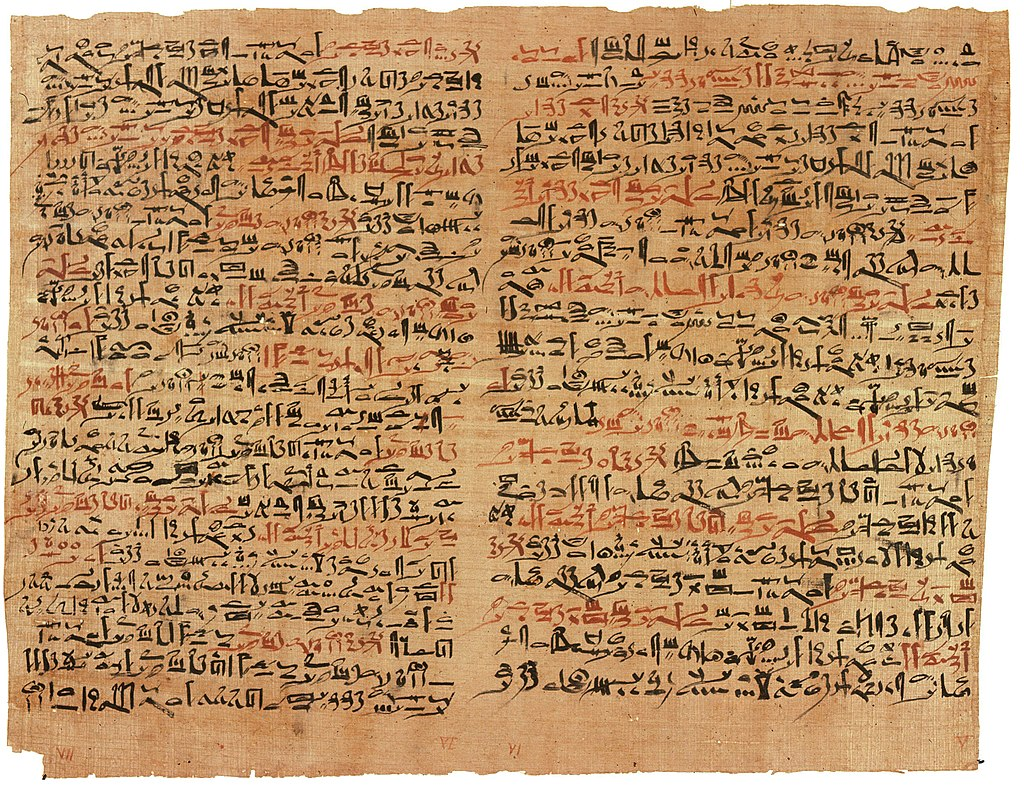
\includegraphics{YOURNAME/images/Edwin_Smith_Papyrus_v2.jpg}
	\caption[]{Edwin Smith Papyrus From \cite{van_middendorp_edwin_2010}}
	\labfig{}
\end{marginfigure} 

One of the areas that has seen exponential technological revolution is the field of medicine. Throughout the ages, humans have sought to understand their bodies, improve their daily lives, and increase longevity. The earliest traces of medical practice date back to antiquity, with civilizations such as the Egyptians, Greeks, and Romans. For example, the Edwin Smith Papyrus (Fig 1.1), dating back to around 1600 BC \cite{van_middendorp_edwin_2010}, is one of the oldest known medical documents and addresses various medical conditions and procedures. The Renaissance and the Scientific Revolution marked a period of significant medical innovation, with figures like Andreas Vesalius (Fig 1.2), who revolutionized anatomy \cite{zampieri_andreas_2015}, and Ambroise Paré. The 19th and 20th centuries represent an essential period of medical innovation with the development of vaccination by Louis Pasteur or the advent of modern surgery and medical imaging techniques. Medical innovations continue to emerge and represent a continuous trajectory of evolution.

\begin{marginfigure}[-5.5cm]
	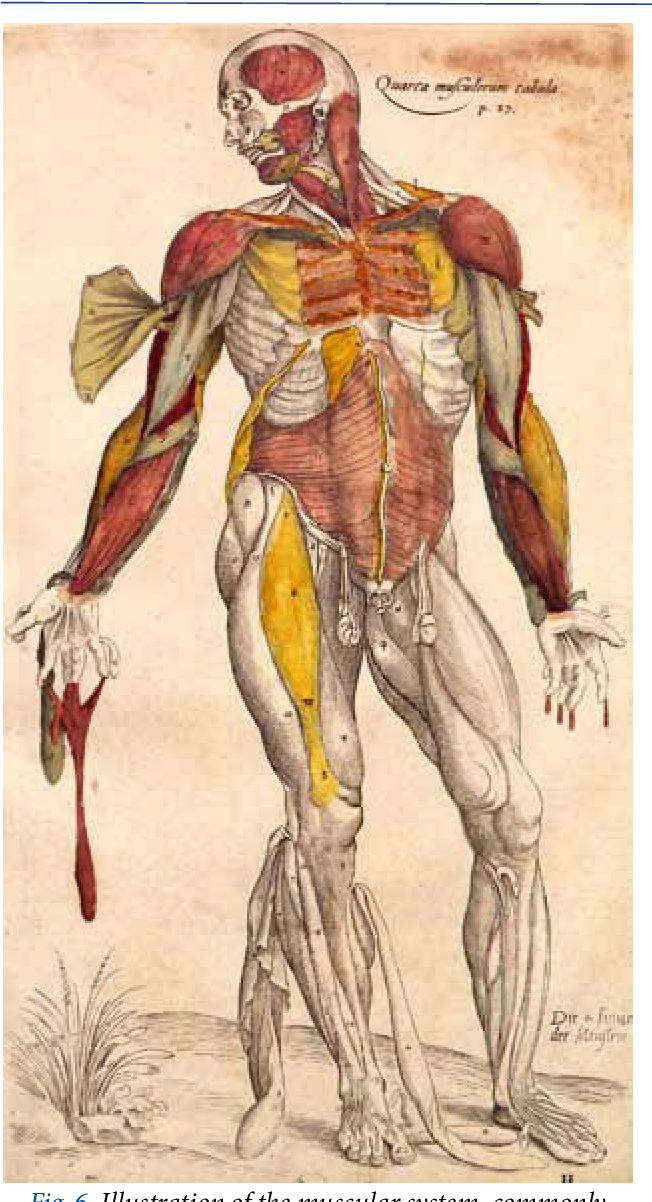
\includegraphics{YOURNAME/images/fig 1.2.png}
	\caption[]{A 16th-century Representation of human anatomy by Andreas Vesalius}
	\labfig{}
\end{marginfigure} 

Among these medical innovations, one of the most significant is the field of prosthetics, which seeks to replace, support, or enhance a lost functionality or severely damaged part of the human body. The emergence of early prosthetics dates back to antiquity, with archaeological discoveries in Egypt revealing the existence of prostheses dating back over 3,000 years \cite{noauthor_prosthesis_2023}. Examples include artificial toes and fingers made of wood and leather (Fig 1.3). Although rudimentary, they testify to the ingenuity and perseverance of humanity in overcoming challenges related to injuries and amputations. The field has seen significant advancements in recent decades thanks to rapid progress in engineering, biomechanics, robotics, and neurology. These advancements have led to sophisticated prostheses replicating movements and functionalities similar to human limbs.

\begin{marginfigure}[-5.5cm]
	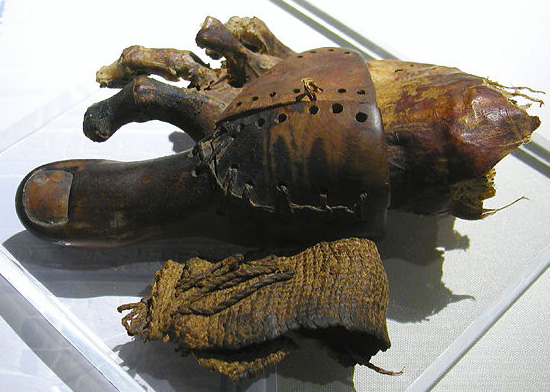
\includegraphics{YOURNAME/images/fig 1.3.jpg}
	\caption[]Egyptian foot prosthesis over 3000 years ago From \cite{noauthor_prosthesis_2023} 
	\labfig{}
\end{marginfigure} 

%\begin{marginfigure}[-5.5cm]
    %\centering
	%\includegraphics[width=0.8\linewidth]{vivien/images-vivien/02_images/LCD.png}
	%\caption[]{Waveshare round LCD module display. From \cite{KubiiLCD}}
	%\labfig{}
%\end{marginfigure} 

Numerous prostheses exist today, varying based on their design, components, and functionality. The main categories include:
Passive Prostheses: These are primarily aesthetic devices designed to replace a missing part of the body visually.
Mechanical Prostheses Mechanical components, such as joints and cables, are used to restore the functionality of a body part.
Myoelectric Prostheses: Controlled by electrical signals generated by the wearer's muscle contractions. Electrodes capture the user's unique and natural movements, reproducing them with simple muscle contractions, enabling more complex and natural movements. They are commonly used for arm and hand prostheses. COAPT has developed a myoelectric control device for upper limb prostheses. This controller is compatible with various prosthetic brands, including Ossür, Psyonic, and Taska. Instead of focusing on the prosthetic design, this company specializes in creating myoelectric control devices \cite{noauthor_coapt_nodate}.
Hydraulic and Pneumatic Prostheses: These use fluids (liquids or gases) to create fluid and controlled movements.
Bionic prostheses incorporate advanced electronic components and sensors to replicate movements and functionalities similar to a human limb’s. A notable example is PSYONIC \cite{noauthor_psyonic_nodate}, which develops bionic prostheses. Using sensors, their prosthesis sends vibrations to the user, allowing them to feel and understand the actions performed with the prosthesis. Furthermore, this prosthesis combines various production methods, such as 3D printing, silicone injection, and CNC machining \cite{noauthor_advanced_nodate}. This approach makes the prosthesis versatile, high-performing, and durable.

In conjunction with prostheses, two significant domains of technological innovation are emerging: haptic and bio-patches. These elements, integrated into prostheses, represent avenues for exploration.

The earliest references to haptic can be found in ancient texts from ancient Greece and China, where philosophers and physicians began to explore the senses, including the sense of touch. For example, Aristotle wrote about tactile perception in his work "De Anima" (On the Soul). The term "haptic" was introduced in the 20th century to refer to studying the sense of touch. The field of haptic has seen significant development during this century, especially with the emergence of tactile technology and human-machine interfaces. Today, haptic has become a full-fledged interdisciplinary discipline with applications in virtual reality, robotics, medical simulation, and many others \cite{noauthor_new_nodate}. Haptic is ubiquitous in our environment, and we experience it daily without necessarily being aware. A typical example can be found in our smartphones, which go beyond simple vibrations to provide an interactive interface and sensory feedback to users during interactions with applications \cite{interhaptics_haptics_2021}. This is notably the case with Apple's taptic engines in iPhones. The use of haptic extends to other fields, including the video game industry. Sony has placed great importance on haptic feedback in their PS5 controller to enhance player immersion \cite{noauthor_whats_nodate}. Additionally, startups like Actronika are dedicated to developing haptic technology in virtual reality, particularly with their skinetic suit, offering new gaming experiences \cite{noauthor_skinetic_nodate}.

In the 1970s, the first work on bio-patches was carried out in medicine, particularly in developing skin patches for controlled drug release. These patches were used to administer drugs continuously and controlled through the skin, such as the patches from Purdue University \cite{service_new_nodate}. Bio-patches designed for the heart are also manufactured using 3D printing technology, an innovation developed by the University of Sydney. After scanning the patient's heart, the team creates a 3D model of the area requiring transplantation and then designs a specific cardiac patch to cover the damaged area \cite{noauthor_mending_2020}. Today, bio-patches are gaining popularity and diversifying. They are increasingly used for home monitoring, telemedicine, and rehabilitation applications.

\section{Research Domain}
The research topic of this thesis lies in the domain (of wearable technologies) of DIY and prothesis innovation. Several disciplines - haptic, design and modeling, and bio-materials science - intertwine, making this research topic a multidisciplinary field.

Haptics and the idea of improving prosthesis is at the base of this project. Haptic technology refers to the study and development of technologies that enable a user to receive touch-based feedback through a device. This feedback can be in the form of vibrations, pressure changes, or other physical sensations that simulate touch or provide additional information about the device's actions.

Engineering design and modeling are essential to innovation, combining creativity and precision. The invention extends beyond aesthetics; it involves creating products, systems, and processes that meet requirements effectively, efficiently, and ethically. At the same time, modeling enables us to simulate and analyze complex systems before they are implemented, to predict their behavior, identify potential problems, and optimize performance.

The field of bio-materials is interdisciplinary, drawing on knowledge from materials science, biology, medicine, and engineering. Bio-materials research aims to develop new materials and technologies to improve health outcomes and quality of life for people with various medical conditions. It allows the understanding of the properties of the materials, allowing a better exploitation of them.

\section{Problem statement}
The wide range of demands and technological possibilities for prosthesis development offers many design, improvement, and innovation opportunities. However, the complexity, standards, cost, and rigor required in this field can make technological innovation and accessibility difficult. To meet this challenge, design tools and methods are needed to simplify prosthesis innovation and enable a first step towards haptic. Indeed, innovation in haptic and prosthetics can present particular difficulties for people unfamiliar with these fields.

\section{Research approach}
Firstly, It begins with an ethical exploration, seeking to understand today's technological accessibility. And starts a reflection on emerging challenges and possible solutions.

Then, it explores how manufacturing technologies and processes can be used to innovate, their use, and applications. It reviews the state of the art and related works in the various fields covered in this paper, their use cases, and limitations, thus increasing knowledge and experimental possibilities...

Finally, a prototyping and testing approach is implemented. A prototype is built and subjected to mechanical assessments and user testing to identify issues and understand needs. This process is repeated until the final version best meets the specified requirements and challenges.

\section{Scientific contribution}
This thesis makes the following contributions :

\textit{Fabrication method}

\item 1. Contribute to the DIY design of a low-cost haptic kit for prostheses with different components, design methods, and uses.
\item 2. Contribute to the design of bio-patches with a method accessible to all and bio-degradable materials.

\textit{Methodological contribution}

\item 1. Contribute to systematically exploring design and prototyping possibilities through different materials and methods for fabricating prostheses or bio-patches.

\textit{Empirical contribution}

\item 1. Proposing an in-depth study of four low-cost materials for prototyping both bio-sourced, water-based, and biodegradable patches: alginate, gellan, gelatin, and glycerine. 
\item 2. Explore how haptic components and prostheses can be combined to create functional interactive devices.
\item 3. Proposes an ethical reflection on technological accessibility at different levels.

\section{Structure of the Thesis}
This thesis revolves around using haptic for prosthetics and its technological accessibility. Chapter 1 is an ethical reflection on technical accessibility at different scales and provides a current overview. Chapter 2 introduces the field of haptic, various related components, and how to use them, offering an overview of haptic-based technologies and research. Chapter 3 focuses on prosthetic and bio-patch design, offering DIY-based solutions. It provides an overview of different prosthetics and the implementation of haptic in them and describes previous work on bio-materials and bio-patches. Finally, this thesis concludes the work and summarizes the discoveries and contributions.